% !TEX root = ./main.tex
% Activation Record
% ======================================================
\par \noindent 活动记录 = 栈帧。
函数调用:1. Push arguments;2. Push return address;3. Save caller-save registers;4. Jump to called function。
被调用函数:1. \texttt{push rbp},\texttt{mov rbp, rsp};2. Save callee-save registers;3. Allocate space for local variables。
函数返回:1. Restore callee-save registers;2.\texttt{mov rsp rbp},\texttt{pop rbp};3. Pop return address;4. Jump back to caller。

\par \noindent 块结构:在允许嵌套函数声明的语言(如 Tiger)中,内部函数可以使用在外部函数中声明的变量,实现方式:

\par \noindent Static link:每次调用函数 g 时,可以将指向静态包围 g 的函数的栈帧的指针在栈中传递给 g(这个指针就是 static link)。
每个函数都带有其嵌套深度的注释,当深度为 $n$ 的函数访问在深度为 $m$ 的函数中的变量时,向上爬 $n-m$ 个链接以访问适当的活动记录。
优点:参数传递时额外开销小;缺点:访问非局部变量时需要向上爬静态链接链,每个变量访问需要一条链,链的长度等于变量声明函数和使用函数的嵌套深度之差。

\par \noindent Lambda Lifting:当 f 调用 g 时,f 中实际访问的每个变量都作为额外参数传递给 g。

\par \noindent Display:可以维护一个全局数组(称为 display),display[i] = 指向最近进入的、其静态嵌套深度为 i 的过程的栈帧的指针。

\begin{figure}[H]
    \centering
    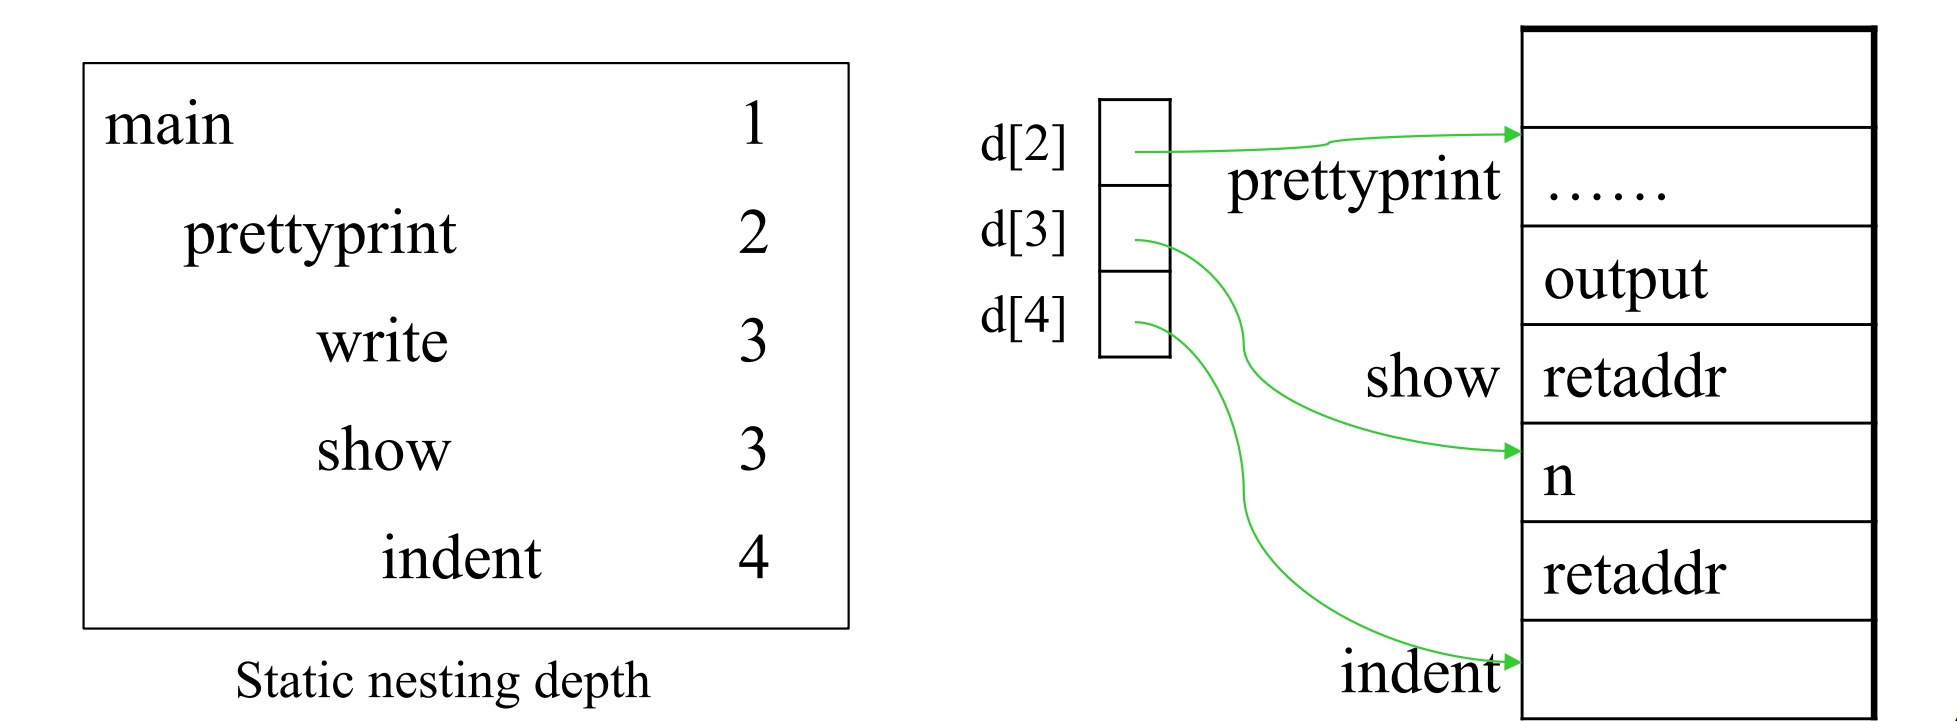
\includegraphics[width=0.8\linewidth]{figures/ar1.png}
\end{figure}

\begin{figure}[H]
    \centering
    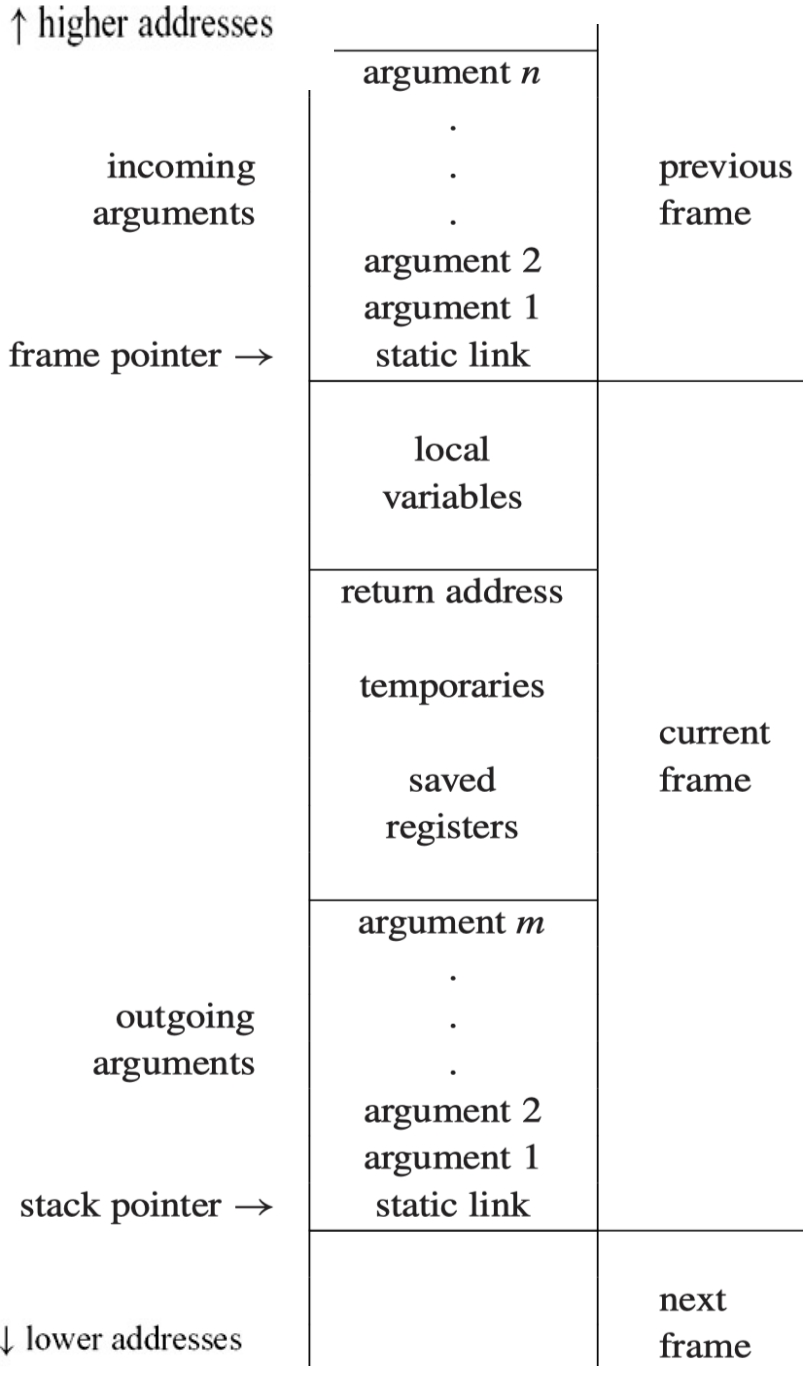
\includegraphics[angle=90, width=0.8\linewidth]{figures/ar2.png}
\end{figure}